%%%%%%%%%%%%%%%%%%%%%%%%%%%%%%%%%%%%%%%%%%
\section{Heat transfer in packed beds} \label{sec:modeling-heat-transfer}
%%%%%%%%%%%%%%%%%%%%%%%%%%%%%%%%%%%%%%%%%%
In our analysis of the momentum of packed beds, we focused entirely on the exchange of momentum between a fluid passing through a packed bed. The mechanics of contacting particles will be dealt with entirely within the framework of the discrete element method, to be discussed in \cref{sec:modeling-dem}. But now as we move to analyze the heat transfer in a packed bed, we will consider both inter-particle modes of heat transfer as well as particle-fluid convection. 


\begin{figure}[t]
	\centering
	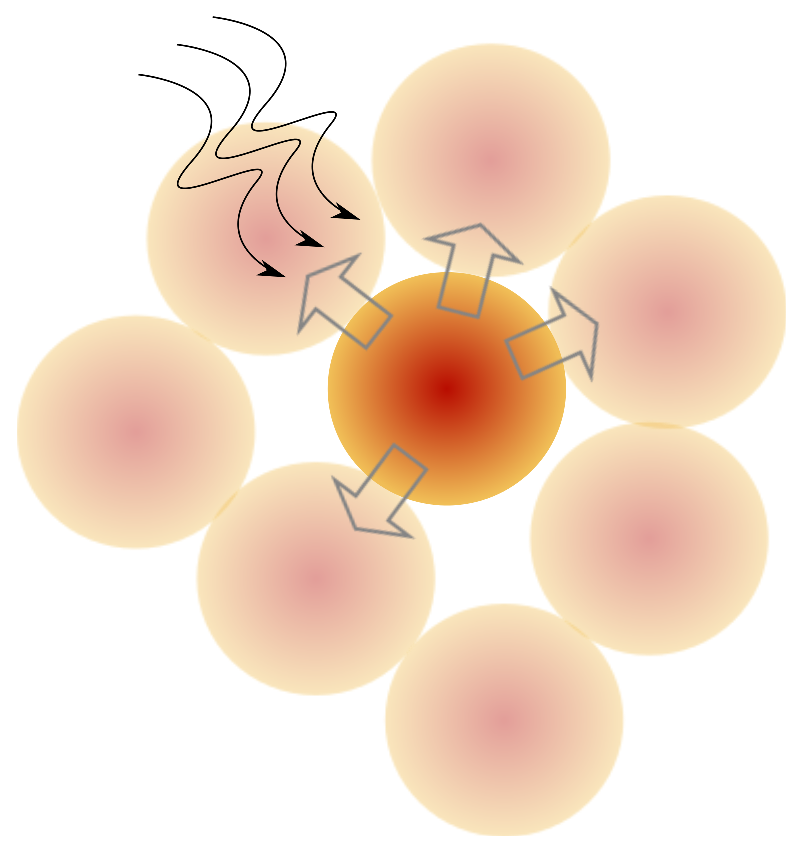
\includegraphics[width=0.35\textwidth]{chapters/figures/pebble-complete-heat-transfer}
	\caption{An illustration highlighting a single particle transferring energy into a passing fluid and neighboring particles in the ensemble.}\label{fig:peb-comp-ht}
\end{figure}

Looking at the particle highlighted in Fig.~\ref{fig:peb-comp-ht}, we see many pathways for heat to be transferred inside the ensemble. The most significant are:

\begin{enumerate}
\item Conduction through the contact area between contacting particles.
\item Conduction through the stagnant fluid between near, non-contacting particles.
\item Conduction through the stagnant fluid between contacting particles.
\item Advection of energy by the fluid to contacting- and downstream particles.
\item Radiation between the surfaces of contacting particles.
\item Radiation between particles of adjacent voids.
\item Heat generation internally in the particle.
\end{enumerate}

We will address the inter-particle conduction in \cref{sec:ht-pebble-conduction} wherein we derive a formula for heat conductance between contacting, elastic spheres. The complex interaction of energy in a particle with a fluid (conduction through film regions, convection with passing fluid, etc.) will all be dealt with using correlations for packed beds; this is done in \cref{sec:particle-convection}. We will briefly discuss some literature where researchers have dealt with the radiation between particles in a packed bed but do not include the terms in our current models. Finally, the last mode of heat transfer is trivially accounted for with a heat source term,

\begin{equation}\label{eq:nuclear-heating-term}
	Q_g = q'''V
\end{equation}

where $q'''$ is a known volumetric heating rate and $V$ is the volume of our particle. In practice, we will know a volumetric heating rate from the location and geometry of the solid breeder volume. The volume of the sphere is $V = \frac{\pi}{6} d_p^3$.

In the following sections we will expand upon the details of the modes of heat transfer considered for our packed beds. They forms of equations used will be written in a way as to be easily implemented directly into the DEM computational framework, to be discussed later in \cref{sec:modeling-dem}.

% The transient energy balance for an irradiated pebble, shown in Fig.~\ref{fig:peb-comp-ht}, in a packed bed with flowing interstitial gas is given by Eq.~\ref{eq:single-pebble-energy},

% \begin{equation}\label{eq:single-pebble-energy}
% 	\rho V C \frac{\mathrm{d}T}{\mathrm{d}t} = \dot{Q}_g + \dot{Q}_\text{conduction} + \dot{Q}_\text{convection} + \dot{Q}_\text{radiation}
% \end{equation}



%%%%%%%%%%%%%%%%%%%%%%%%%%%%%%%%%%%%%%%%%%
\subsection{Inter-particle heat conduction}\label{sec:ht-pebble-conduction}

When two particles come into contact, energy is transmitted through their region of contact. For this discussion, we assume the particles are spherical, elastic, in vacuum, and we neglect radiation transfer between them. If the two particles are at temperatures $T_i$ and $T_j$ we can quantify the amount of energy transferred between them with a commonly used practice of a contact conductance, $H_c$:
\begin{equation}\label{eq:pebble-conduction-heat-transfer}
	Q_{ij} = H_{c}(T_i - T_j)
\end{equation}

The subscripts are omitted for clarity, but obviously there is a unique $H_c$ per pair of contacting particles. We note that the heat conductance, unlike standard heat transfer coefficients, has units of \si{W/K}.

Batchelor and O'Brien\cite{Batchelor1977} developed a formulation of similar form and then made the brilliant observation that the temperature fields in the near-region of contacting spheres are analogous to the velocity potential of an incompressible, irrotational fluid passing from from one reservoir to another through a circular hole in a planar wall separating the two reservoirs. With the analogy, they could make use of the fluid flow solution to write the total flux across the circle of contact just as Eq.~\ref{eq:pebble-conduction-heat-transfer} with the heat conductance as

\begin{equation}\label{eq:batchelor-pebble-conductance}
	H_c = 2k_ra
\end{equation}

where $k_r$ is the conductivity of the contacting solids and $a$ is the radius of contact. In \cref{sec:hertz-theory}, with Hertz theory we found the contact radius in terms of the contact pressure. Here, we give the radius in terms of the compression force acting on the bodies,

\begin{equation}
	a =  \left(\frac{3}{4}\frac{R^*}{E^*}\right)^{1/3}F_n^{1/3}	
\end{equation}

as before, $\frac{1}{E^*} = \frac{1-\nu_1^2}{E_1} + \frac{1-\nu_2^2}{E_2}$ and $\frac{1}{R^*} = \frac{1}{R_1} + \frac{1}{R_2}$. 

In the development of Eq.~\ref{eq:batchelor-pebble-conductance}, Batchelor and O'Brien had assumed the two contacting spheres to be of equal conductivity, $k_r$. Cheng, et al.\cite{Cheng19994199} proposed a slightly modified conductance which allows for contacting materials of different thermal conductivity. They have,

\begin{equation}\label{eq:cheng-modification-batchelor}
	H_c = 2k^*a = 2k^* \left(\frac{3}{4}\frac{R^*}{E^*}\right)^{1/3}F_n^{1/3}
\end{equation}

where $\frac{1}{k^*} = \frac{1}{k_i} + \frac{1}{k_j}$. As well as being a more general, flexible formulation, the models analyzed by Cheng, et al.\cite{Cheng19994199} are in good agreement with experiments. In the DEM numerical structure, we use the form given by Eq.~\ref{eq:cheng-modification-batchelor}.

Furthermore, Batchelor and O'Brien developed Eq.~\ref{eq:batchelor-pebble-conductance} with the assumption of two contacting particles in vacuum but, once developed, showed\cite{Batchelor1977} that this form is still valid when immersed in a fluid providing that the thermal conductivity ratio of solid and fluid is well above unity. The condition is expressed as,

\begin{equation}\label{eq:conductance-validity-fluid}
	\frac{ k_r }{ k_f } \frac{a}{R^*} \gg 1
\end{equation}

The term $\frac{a}{R^*}$, from \cref{sec:hertz-theory}, is necessarily much less than 1 for Hertz theory to be applicable. Thus for fluid in vacuum, the condition is identically satisfied but we must consider inaccuracies if we introduce an interstitial fluid with low conductivity ratios; for lithium ceramics in helium, the ratio is approximately $\frac{k_r}{k_f} \approx 10$.

As we step back from the contact of a single pair of particles and consider a particle in an ensemble with many contacts, we must again consider the validity of applying Eq.~\ref{eq:cheng-modification-batchelor} at each contact. Vargas and McCarthy\cite{Vargas2002a}, proposed introducing a conduction Biot number to relate resistance to heat transfer internal to the particle with the resistance between particles. We use the following form

\begin{equation}
	\Bi_c = \frac{H_c}{k^* d_p} = 2\frac{a}{d_p}
\end{equation}

Then if $\Bi_c \ll 1$, the individual energy transferred between each point of contact can be decoupled. The Biot number criteria is already satisfied for Hertz theory to be valid; having assumed that $\frac{a}{d_p} \ll 1$. Therefore the total heat transferred out of a single particle with $Z$ contacts is the summed contribution of individual contacts, 

\begin{equation}
	Q_i = \sum_j^Z Q_{ij}
\end{equation}

The contact conductance we use, Eq.~\ref{eq:cheng-modification-batchelor}, which is built upon the solution of Batchelor and O'Brien\cite{Batchelor1977}, has been implemented by others in a variety of studies\cite{Vargas2001, Chaudhuri2006, Zhou2009,Cheng19994199}. However, in many other fields, the researchers are interested in such things as the parallel conduction through a stagnant interstitial gas\cite{Bu2013} or the temporary conduction during impact of fluidized beds\cite{Zhu2008,Zhang2011,Wu2011,Li2000}. In such cases, the formula for conductance can be quite different but are not appropriate for the physics of our packed beds.

% Nevertheless, for the packed beds of ceramic spheres for which we are working towards modeling, the heat conductance of Eq.~\ref{eq:cheng-modification-batchelor} is an appropriate and valid form. The interstitial gas, be it stagnant or moving, will be incorporated the influence of an interstitial gas, it will be done in such a way as to leave the DEM heat transfer intact and only add an energy source term to stand in for the interaction with the fluid. The details will be discussed in \cref{sec:cfdem-heat-transfer}, but for now we conclude with a solid conduction theory that will be implemented in the discrete element method computations.
\section{Nusselt number for spheres in packed beds}\label{sec:particle-convection}
\subsection{Convection by interstitial gas}

Engineers have paid considerable attention to the calculation of convective heat transfer in packed beds. Correlations for determining the Nusselt number of a sphere in dilute and dense packings over a range of Reynolds and Prandtl number are available. We will cover the detail of many of these correlations in \S\ref{sec:}. The methods all come down to calculating Nusselt number to find the heat transfer coefficient and then computing the rate of heat transfer from convection as

\begin{equation}
	\dot{Q}_\text{convection} = -hA(T_s-T_f)
\end{equation}

where $T_s$ is the temperature of the solid with surface area, $A$, and $T_f$ is the local bulk temperature of the passing fluid. The negative sign is to maintain convention that energy transfer into the solid is positive.

\subsection{Radiative transfer with neighboring particles}

The temperatures expected in the solid breeder are high enough that we can not a priori neglect radiation. The radiation exchange between contacting neighbors in a packed bed becomes extremely complex due to the local and semi-local nature of radiation. A standard approach to treat radiation exchange between surfaces is to consider the view factor between them. In a dense, randomly packed bed of spheres the computation of view factors between pebbles can be done via a method such as that proposed Feng and Han\cite{Feng2012}. Ideally, we could show this mode of heat transport is negligible compared to the others already discussed.

In ceramic breeder designs, the tritium breeding volume is rarely more than \si{2 cm} wide with pebbles that are, generally, \si{1 mm} in diameter. The maximum expected temperature in the breeding zone is about \si{1000 K}, roughly at the centerline of the \si{2 cm} width. The walls of the coolant must be held below the operable steel temperature of roughly \si{700 K}. This works out to a \si{300 K} differences spanning 10 pebble diameters. From this we can make a first-order approximation of \si{30 K} difference between neighboring pebbles. At the elevated temperatures, an estimate for the radiation exchange between two pebbles (allowing them to act as black bodies for this approximation) is

\begin{equation}
	\dot{Q}_\text{radiation} = \sigma A \left(T_\text{max}^4 - (T_\text{max}-30)^4\right) \approx 0.022\si{W}
\end{equation}
 
 which is the highest amount of radiation exchange we might expect between pebbles. Even though we will neglect this mode of heat transfer for now, after reviewing some of the packed bed heat transfer results we may find that this quantity of energy transfer is not negligible and future versions of the model would have to account for it.
%%%%%%%%%%%%%%%%%%%%%%%%%%%%%%%%%%%%%%%%%%
